%!TEX TS-program = xelatex
%!TEX encoding = UTF-8 Unicode
\documentclass[17pt]{memoir}

\usepackage{xltxtra,fontspec,xunicode}
\defaultfontfeatures{Scale=MatchLowercase}
%\setromanfont[Numbers=Uppercase]{Hoefler Text}
%\setmonofont[Scale=0.90,Ligatures=NoCommon]{Courier}

\setmainfont[BoldFont={OpenDyslexic3-Bold.ttf} ]{OpenDyslexic3-Regular.ttf}
%\setmainfont[
% BoldFont={OpenDyslexic-Bold.otf}, 
% ItalicFont={OpenDyslexic-Italic.otf},
% BoldItalicFont={OpenDyslexic-BoldItalic.otf}
% ]{OpenDyslexic-Regular.otf}

%\usepackage{natbib}

\usepackage{hyperref}
\hypersetup{
    colorlinks=true,       % false: boxed links; true: colored links
    linkcolor=black,          % color of internal links (change box color with linkbordercolor)
    citecolor=black,        % color of links to bibliography
    filecolor=blue,      % color of file links
    urlcolor=blue           % color of external links
}

\title{Dyslexia}
\author{Lyron Winderbaum}

\begin{document}

\maketitle



Dyslexia is estimated to occur in 15-20\% of the Australian population, around 10\% being diagnosed with dyslexia and the rest being undiagnosed. Under the conservative assumption that only 10\% of students have dyslexia, any given class of 25 randomly selected students will have \textbf{at least 2 students} with dyslexia with a probability over 70\%. In the more realistic case that 20\% of students have dyslexia, as claimed by the \href{https://dyslexiaassociation.org.au/dyslexia-in-australia/}{Australian Dyslexia Association}, this probability rises to over 97\%. Taking into account the possibility for undiagnosed dyslexia (particularly for students who went through primary school in another country, and students whose dyslexia might be masked by another learning disability), the conclusion is that it is reasonable to conduct ourselves as teachers under the assumption that every one of our classes will have dyslexic students in them, if have identified them or not. 

Knowing that every one of our classes is likely to contain multiple dyslexic students, both diagnosed and undiagnosed, makes strategies for addressing their needs to ensure they have an equal opportunity to learn in our classrooms critical. Many strategies for addressing the needs of dyslexic students would benefit all students anyway, and it makes sense to focus on such strategies both because undiagnosed dyslexia can be the most problematic with the possibility of students blame their difficulties in completing tasks on "being stupid" --- a potentially crippling beleif to a learner. It is also important to be realistic and recognise the pressures on teachers time and attention, and as such it is doubly important to focus on strategies that are easy to implement, take minimal time and effort from teachers, and can be implemented class-wide. Differentiation is important, but can also sometimes require a heavy time-investment from already extremely time-poor teachers. When the same or better outcomes can be acheived through class-wide teaching strategies instead of individualised tailoring, this should be pursued. This second point is particularly important when taking into account the prevalence of dyslexia.

In this report I will cover a number of strategies for making the learning more accessible to students with dyslexia, with a focus on those that can be implemented class-wide and also benefit non-dyslexic students. Each strategy has a different amount of evidence to demonstrate it's effectiveness, and takes a different amount of time and effort to implement. These points will be discussed, and some comments will be made about how some of these apporaches could also be used for indivudually differentiate for particular students with dyslexia in efficient and as effective as possible ways. The remainder of this report wil be structured into the following sections:
\begin{itemize}
	\item Font Size / Typeface
	\item Use of Colour
	\item Portioning Content / Timing
	\item Tailoring Content through Formative Assessment
\end{itemize}

Then maybe I'll talk a little about the research and literature if I have space.

\section*{Font Size / Typeface}

There has been much discussion in the literature about fonts and typefaces that could make reading easier for people with dyslexia. The appeal is obvious --- there is not much that could be easier than simply converting all your resources to a different font, the question is does it really work and if it does, what font works best? There have been several fonts specifically developed and marketed to make reading easier for dyslexic people, notably: \href{https://www.dyslexiefont.com/en/typeface/}{Dyslexie}, \href{http://www.robsfonts.com/fonts/sylexiad}{Sylexiad}, \href{http://www.readregular.com/english/intro.html}{Read Regular} and \href{https://www.opendyslexic.org/}{Open Dyslexic}. Of these Open Dyslexic is the only one free to access, and as such that is the font I chose for this research paper although \cite{Wery2017} found no significant difference in reading time between Open Dyslexic an deither Arial or Times New Roman. 

On \href{https://www.dyslexiefont.com/en/typeface/}{the Dyslexie website} they describe nine features of their font that they believe make it easier to read for Dyslexic people, although they don't provide the evidence for these points. In \cite{Leeuw2010} it was found that Dyslexie font does not increase the reading speed of words, but can reduce some types of reading errors at the cost of increasing other types of reading errors. In contrast, \cite{Marinus2016} found that the Dyslexie font \textbf{can} infact increase reading speed in comparison to Arial, but that this difference can be entirely explained by factors such as letter spacing (which is feature number 9 on \href{https://www.dyslexiefont.com/en/typeface/}{Dyslexie website}\href{https://www.dyslexiefont.com/en/typeface/}{the Dyslexie website}). 

The only study I found to do a broad an objective comparison of many fonts was \cite{Rello2013}, who compared the 12 fonts shown in Figure~\ref{fig:RelloFonts} using eyetracking data to compare reading speed and fixation duration. 

Also, \href{https://www.dyslexicadvantage.org/the-best-fonts-for-dyslexia/
}{https://www.dyslexicadvantage.org/the-best-fonts-for-dyslexia/
}

\begin{figure}

\begin{center}
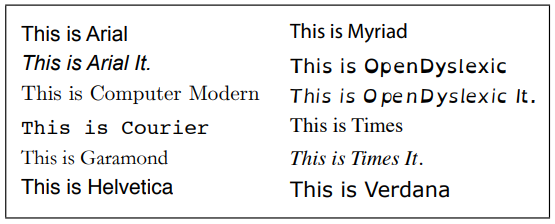
\includegraphics{figures/RolloFonts.PNG}
\end{center}

\caption{Figure 1 of \cite{Rello2013} showing the fonts used in their experiment. \label{fig:RelloFonts}}
\end{figure}


On these issues the literature is divided at best, but there are certain emerging trends which I will attempt to describe here. 


I could add more detail here about why people think these would be effective, including the reasoning on the Dyslexie website before going into the research on why they don't work.


\cite{French2013}
Disfluent font (Monotype Corsiva) cause more cognitive processing due to the font being harder to read, and this causes them to learn and undestand the underlying material better than the control font (Arial).

Use eye tracking to compare 12 fonts. 


To summarise the findings:
\begin{itemize}
	\item Using a larger font size makes reading easier.
	\item Using italics makes reading harder.
\end{itemize}
This is a complicated  typeface of a font may not have much effect, but the spacing settings might.


\section*{Use of Colour}

\cite{Ludlow2006}
\cite{Jeanes1997}
\cite{Wilkins1994}
\cite{Singleton2005}
\cite{Henderson2013}
\cite{Lightstone1999}


\section*{Portioning Content / Timing}

Evidence: Does it work \href{https://blog.dyslexia.com/evidence-based-but-does-it-work/}{https://blog.dyslexia.com/evidence-based-but-does-it-work/}

\section*{Tailoring Content: Formative Assessment}

\href{https://educationtechnologysolutions.com.au/2015/02/10-achievable-strategies-to-tackle-dyslexia-in-your-classroom-and-school/}{https://educationtechnologysolutions.com.au/2015/02/10-achievable-strategies-to-tackle-dyslexia-in-your-classroom-and-school/}

\pagebreak
\section*{References}

What follows is a list of less formal sources used when researching this topic that where not explicitly cited above:
\begin{itemize}
	\item \href{https://www.dyslexia.com/about-dyslexia/understanding-dyslexia/guide-for-classroom-teachers/
}{https://www.dyslexia.com/about-dyslexia/understanding-dyslexia/guide-for-classroom-teachers/
},
	\item \href{https://www.theguardian.com/teacher-network/teacher-blog/2013/sep/09/supporting-students-with-dyslexia-teachers-tips-pupils
}{https://www.theguardian.com/teacher-network/teacher-blog/2013/sep/09/supporting-students-with-dyslexia-teachers-tips-pupils
},
	\item \href{https://educationtechnologysolutions.com.au/2015/02/10-achievable-strategies-to-tackle-dyslexia-in-your-classroom-and-school/
}{https://educationtechnologysolutions.com.au/2015/02/10-achievable-strategies-to-tackle-dyslexia-in-your-classroom-and-school/
},
	\item \href{https://www.dyslexia-international.org/ONL/EN/Course/Welcome.htm
}{https://www.dyslexia-international.org/ONL/EN/Course/Welcome.htm
},
	\item \href{https://blog.capterra.com/teaching-students-with-dyslexia-4-effective-lesson-plans/
}{https://blog.capterra.com/teaching-students-with-dyslexia-4-effective-lesson-plans/
},
	\item \href{https://www.britishcouncil.org/voices-magazine/how-teachers-can-help-learners-dyslexia
}{https://www.britishcouncil.org/voices-magazine/how-teachers-can-help-learners-dyslexia
},
	\item \href{https://www.drgavinreid.com/free-resources/dyslexia-teaching-approaches/
}{https://www.drgavinreid.com/free-resources/dyslexia-teaching-approaches/
},
	\item \href{http://www.dyslexiavictoriaonline.com/how-teachers-can-accommodate-the-dyslexic-student/
}{http://www.dyslexiavictoriaonline.com/how-teachers-can-accommodate-the-dyslexic-student/
},

\end{itemize}

\bibliographystyle{abbrv}
\bibliography{citations} 

\end{document}


